%!TEX root = doc.tex
\section{The \apiname{} API} % (fold)
\label{sec:proposal}

%% Intro to the proposal
% Framework limitations issues
The modelling of agent-based systems can be accomplished using one of the wide number of available platforms. In order to benefit from different features, modelling the same MAS in different tools may be necessary.
% The main goal of this proposal
The API we propose is the direct result of an undergoing project to solve such need. More specifically, we propose a way to easily create JADE-like simulations based solely on the Repast Symphony platform.

The main feature of \apiname{} is the fact that it enables the development of FIPA-compliant MABS in Repast.
% A secondary objective
A fundamental goal that has also been taken in consideration in the framework's architecture is to be able to seamlessly convert between the two frameworks.
% Conclusion and intro to the section objective
In this section we describe \apiname{}'s architecture thoroughly, while comparing our design decisions with those of JADE.
% [citation needed: is conversion a real need?]


\subsection{\gls{FIPA} Specifications}

% Brief intro
As previously mentioned, \apiname{} closely follows JADE's architecture.
% The DF Agent Description in the api
Our API implements the DF Agent Description used to filter DF searches. The focus of our tool is the development of local simulations (as opposed to distributed). As such, a single DF exists in each simulation. \apiname{}'s implementation of the MTS is simplified as well due to the absence of a distributed infrastructure considering that agent address resolution is unnecessary. The AMS contains a mapping of all AIDs to their respective agent objects, which is used by the MTS when delivering messages.
% The ACL message in the api
Our implementation of the ACL Message is slightly simpler than the one found in JADE, focusing on the most commonly used elements (the ones highlighted in Table \ref{tab:fipaACLMessage}).

% The interaction protocols in the api
\apiname{}'s initial focus was the incorporation of \gls{FIPA} Interaction Protocols in Repast, but now includes this agent management infrastructure. At the present time, we selected a few of the most common protocols, following JADE's implementation, to include in \apiname{}.
% The specific protocols
These are the ``request-like'' Achieve Rational Effect (AchieveRE) protocol, the Propose protocol and the Contract Net protocol. The AchieveRE encompasses multiple \gls{FIPA} protocols, namely Request, Query, Request-When, Recruiting and Brokering protocols, as defined in JADE's documentation.


\subsection{Agent Execution}

% Agent execution in JADE and Repast
JADE agent execution can be concurrent and parallel, since JADE supports distributed and multi-threaded agent systems. Agent execution in Repast, on the other hand, is not concurrent. Repast uses a time-share type of execution, granting each agent the right to perform its tasks until they finish them, in sequence, but in no particular order.

% Agent execution in the API
When integrating agent behaviours in \apiname{}, including those related with interaction protocols, it was necessary to make adaptations to JADE behaviours implementation, in order to take Repast's concept of time into account. Even though a local application can take advantage of direct method invocation, for the sake of compatibility with JADE, communication in \apiname{} is also made asynchronously.

Figures \ref{fig:com-example-jade} and \ref{fig:com-example-repast} represent a scenario where two agents send a message to a third one who then replies. In Repast (Fig. \ref{fig:com-example-repast}), messages are delivered to agent C's message queue, and processed only in C's turn. In JADE (Fig. \ref{fig:com-example-jade}), messages can arrive concurrently. Their arrival triggers an event and they are processed right away. In this case, agent C handled the messages as they arrived and issues the respective replies.

\begin{figure}
	\centering
	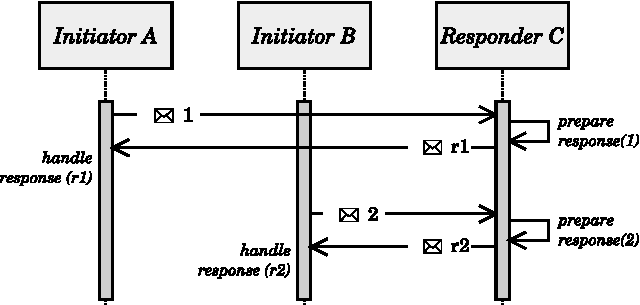
\includegraphics[width=3.0in]{figures/tickExample2.pdf}
	\caption{
		Communication example in JADE. Agents are executed concurrently or in parallel. 
	}
	\label{fig:com-example-jade}
\end{figure}

\begin{figure}
	\centering
	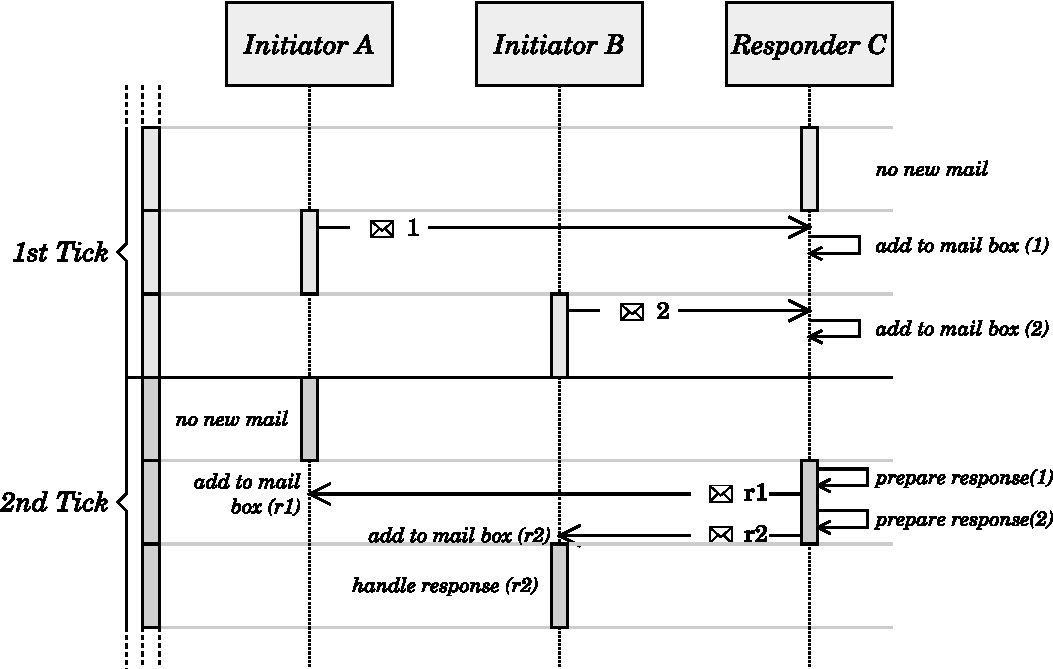
\includegraphics[width=3.8in]{figures/tickExample.pdf}
	\caption{
		Communication example in Repast using \apiname{}.
	}
	\label{fig:com-example-repast}
\end{figure}

While the diagram above represents the agents a scheduled objects, their behaviours are the ones being scheduled. It is worth noting that the order by which Repast executes each scheduled behaviour is unpredictable. In fact, it is not guaranteed that all the behaviours of a single agent are executed consecutively. This is the expected execution when working with Repast as well as with JADE (given its multi-threaded nature) and it is up to the programmer to ensure that the application does not rely on the order of execution.

\subsection{Architecture}

Figure \ref{fig:arch} illustrates the details of \apiname{}'s architecture. Most concepts represented in this diagram are present in JADE, namely the Agent, ACL Message, Behaviour, MTS and DF service.

An agent in \apiname{} contains a MessageQueue and a set of Behaviours. These have access to the agent who owns them and to its MessageQueue. A behaviour that implements an interaction protocol makes use of MessageTemplates. These are used to retrieve relevant messages in each step of the protocol. The MessageTemplates are updated while the protocols go through their different states.

The DFService, as described before, provides the yellow page service. Agents can register or deregister themselves in the DF as well as perform searches. While tasks can be performed during agent setup, in runtime they are typically executed inside Behaviours.

To follow JADE-like communication, ACL Messages carry agent identifiers (AID) for senders and receivers. These AIDs are returned by the DF as search results and are resolved to an agent by the MTS when sending a message. In \apiname{} the MTS keeps a mapping of AIDs to agents for easier access.

The ``plug-in points'' of the API are the Agent, the Behaviour and their derived classes. The API also supports direct access to the DFService. In Figure \ref{fig:arch} all protocol definitions are implied by the generic sub-classes ``ProtocolInitiator'' and ``ProtocolResponder''. 

\begin{figure}[h]
	\centering
	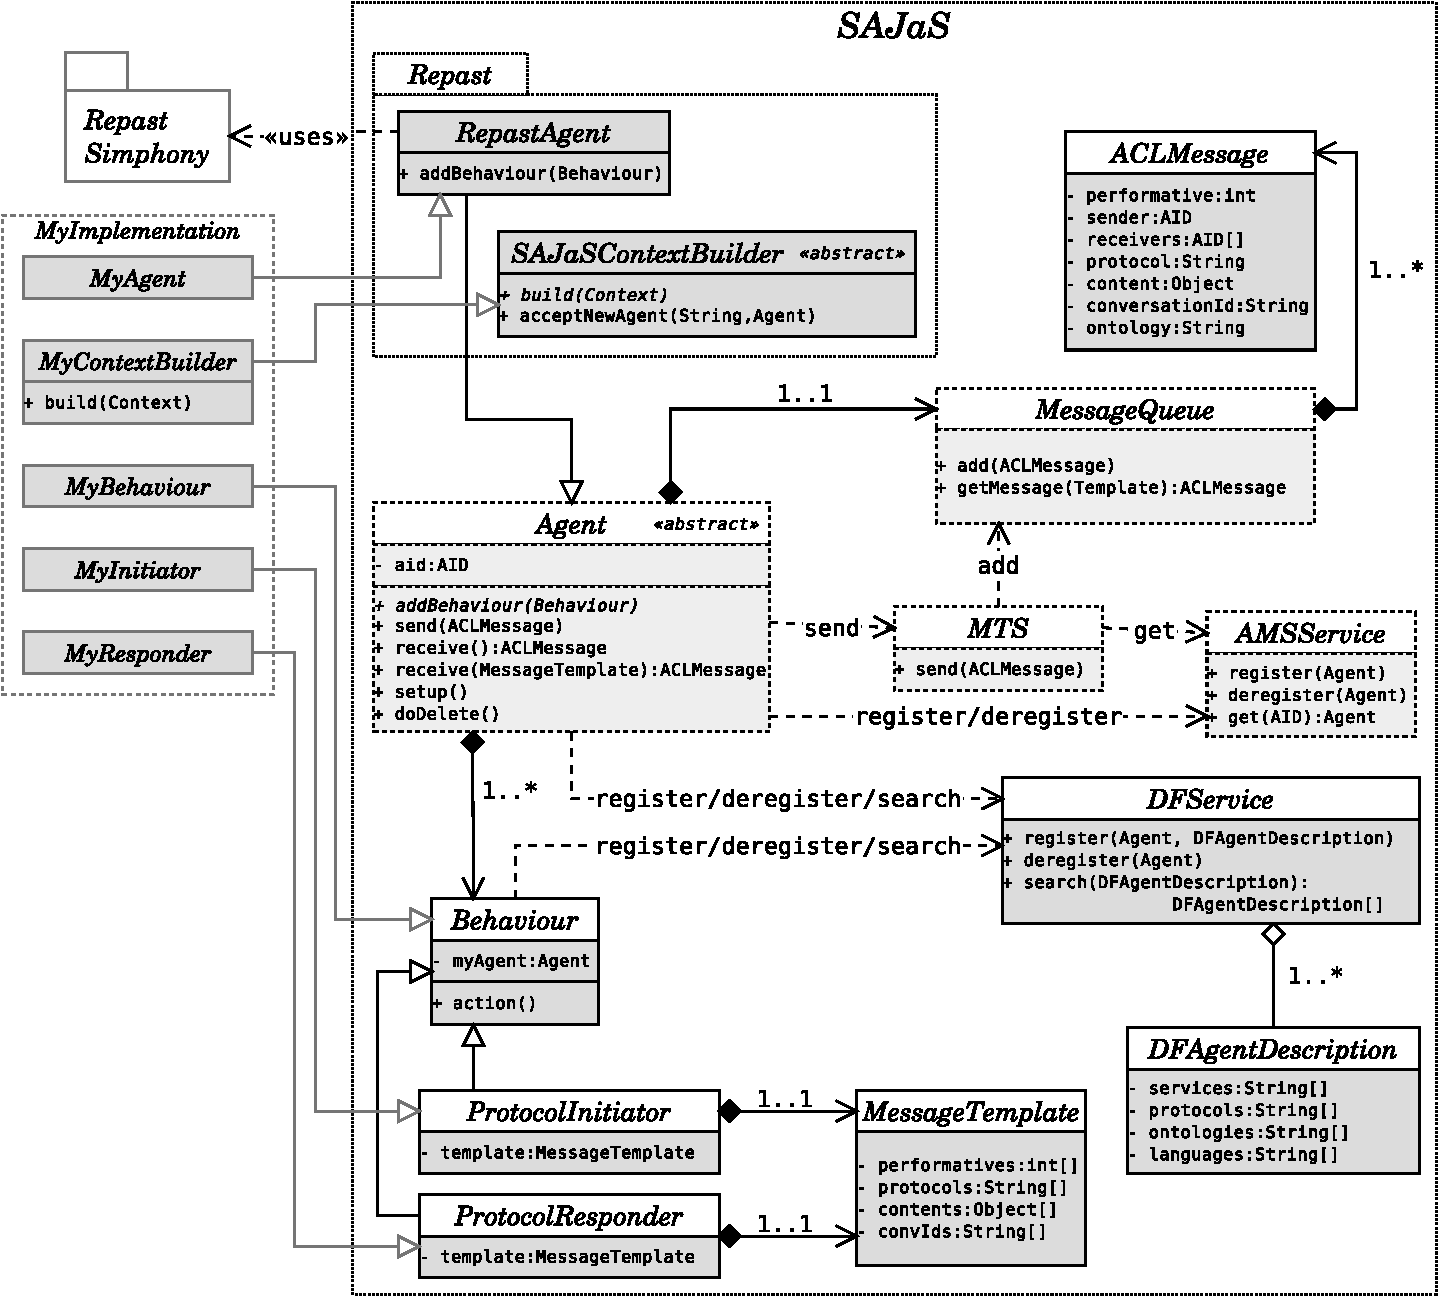
\includegraphics[width=\linewidth]{figures/repacl_arch.pdf}
	\caption{Detailed architecture of \apiname{}. The classes with doted border are internal.}
	\label{fig:arch}
\end{figure}

\subsection{Using Repast}

Even though the API is fairly generic in its architecture, allowing its integration with different frameworks, the main candidate for integration is Repast Simphony. As such, we include an implementation of the AbstractAgent called RepastAgent. It handles the logic of scheduling the behaviour and managing of the Context. The Context is a Repast structure that contains the set of objects to be scheduled. In Figure \ref{fig:arch}, the Context in the API is a wrapper for the Repast Context.


% section proposal (end)